\documentclass[12pt,a4paper]{article}
\usepackage[polish]{babel}
\usepackage[T1]{fontenc}
\usepackage{lmodern}
\usepackage[utf8x]{inputenc}
\usepackage{hyperref}
\usepackage{url}
\usepackage{graphicx}
\usepackage{listings}
\usepackage{xcolor}

\colorlet{punct}{red!60!black}
\definecolor{background}{HTML}{EEEEEE}
\definecolor{delim}{RGB}{20,105,176}
\colorlet{numb}{magenta!60!black}

\lstdefinelanguage{json}{
    basicstyle=\normalfont\ttfamily,
    numbers=left,
    numberstyle=\scriptsize,
    stepnumber=1,
    numbersep=8pt,
    showstringspaces=false,
    breaklines=true,
    frame=lines,
    backgroundcolor=\color{background},
    literate=
     *{0}{{{\color{numb}0}}}{1}
      {1}{{{\color{numb}1}}}{1}
      {2}{{{\color{numb}2}}}{1}
      {3}{{{\color{numb}3}}}{1}
      {4}{{{\color{numb}4}}}{1}
      {5}{{{\color{numb}5}}}{1}
      {6}{{{\color{numb}6}}}{1}
      {7}{{{\color{numb}7}}}{1}
      {8}{{{\color{numb}8}}}{1}
      {9}{{{\color{numb}9}}}{1}
      {:}{{{\color{punct}{:}}}}{1}
      {,}{{{\color{punct}{,}}}}{1}
      {\{}{{{\color{delim}{\{}}}}{1}
      {\}}{{{\color{delim}{\}}}}}{1}
      {[}{{{\color{delim}{[}}}}{1}
      {]}{{{\color{delim}{]}}}}{1},
}

\title{Landscape Generator\\Inżyniera Oprogramowania}
\author{Artur Bednarczyk, Dawid Grajewski, Tomasz Januszek\\Politechnika Śląska\\Wydział Matematyki Stosowanej\\Informatyka, semestr V}
\date{\today}

\begin{document}
\maketitle
\newpage
\tableofcontents
\newpage
\section{O projekcie}
\subsection{Zespół}
\begin{tabular}{c|l}
Osoba & Główna odpowiedzialność \\
\hline
Artur Bednarczyk & Algorytm generujący kształt terenu, organizacja, dokumentacja \\
Dawid Grajewski & Silnik wyświetlający teren \\
Tomasz Januszek & UI aplikacji, algorytm generujący kształt terenu
\end{tabular}
\subsection{Temat}
\paragraph{Generowanie realistycznych krajobrazów 3D}
Generowanie w języku wysokiego poziomu (nie w generatorach typu Unity) losowych krajobrazów z uwzględnieniem zadanych parametrów: stromizny terenu, poziomu wody, kolorów na danej wysokości lub obszarzem wizualizacja i symulacja przemieszczania kamery.

Bonus: dodanie roślinności (drzewa, krzewy - co najmniej 3 rodzaje) o zadanej częstości i miejscu występowania.

\section{Projekt}
\subsection{Plany i pomysły}
Zgodnie z założeniami projektu, głównym naszym celem jest wygenerowanie losowego krajobrazu, który będzie realistyczny, przy czym nie wykorzystamy gotowych silników typu Unity. Plan jest taki, aby użytkownik mógł podać parametry, zgodnie z którymi zostanie wygenerowany krajobraz oraz miał możliwość zapisania i odczytania wybranego krajobrazu. Chcemy również dodać możliwość wyświetlania dodatkowych elementów, takich jak drzewa, krzewy.
\subsection{UI/UX}
\subsubsection{Zawartość}
UI programu będzie złożone z kilku elementów:
\begin{itemize}
\item Menu - pozwoli na przejście do ustawień generowania, informacji o aplikacji oraz do wczytania wcześniej zapisanego krajobrazu.
\item Ustawienia generowania - pozwoli na ustawienie konkretnych parametrów, zgodnie z którymi zostanie wygenerowany krajobraz. Parametry te to: 
	\begin{itemize}
	\item Stromizna terenu
	\item Poziom wody
	\item Górzystość
	\item Gęstość dodatkowych elementów
	\item Położenie dodatkowych elementów
	\item Rozmiar krajobrazu
	\end{itemize}
	\item Informacje - o aplikacji, autorach
	\item Wygenerowany krajobraz - tutaj użytkownik może się poruszać po obszarze, który został wygenerowany oraz go zapisać.
\end{itemize}
\subsubsection{Projekty UI}
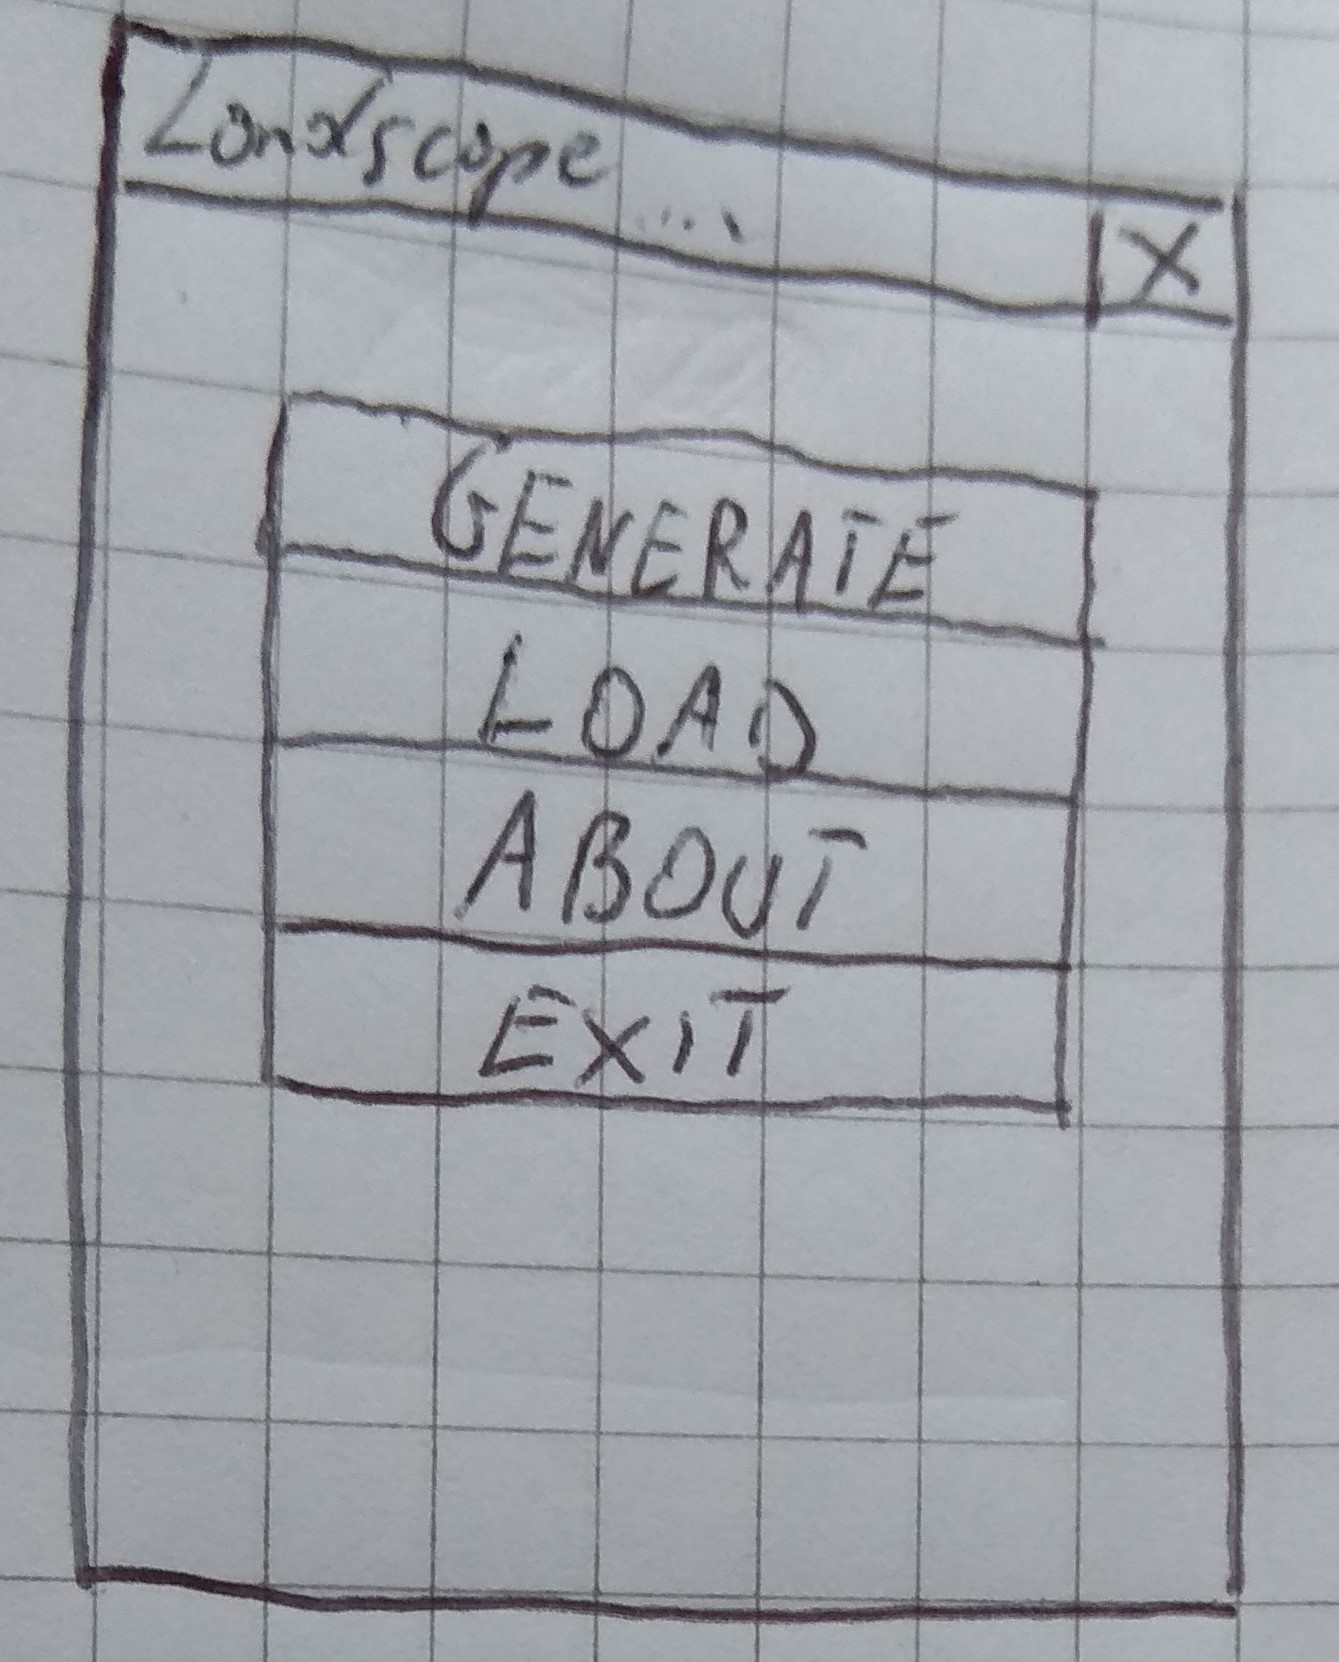
\includegraphics[width=0.5\textwidth]{Images/ui-mainForm.jpg}
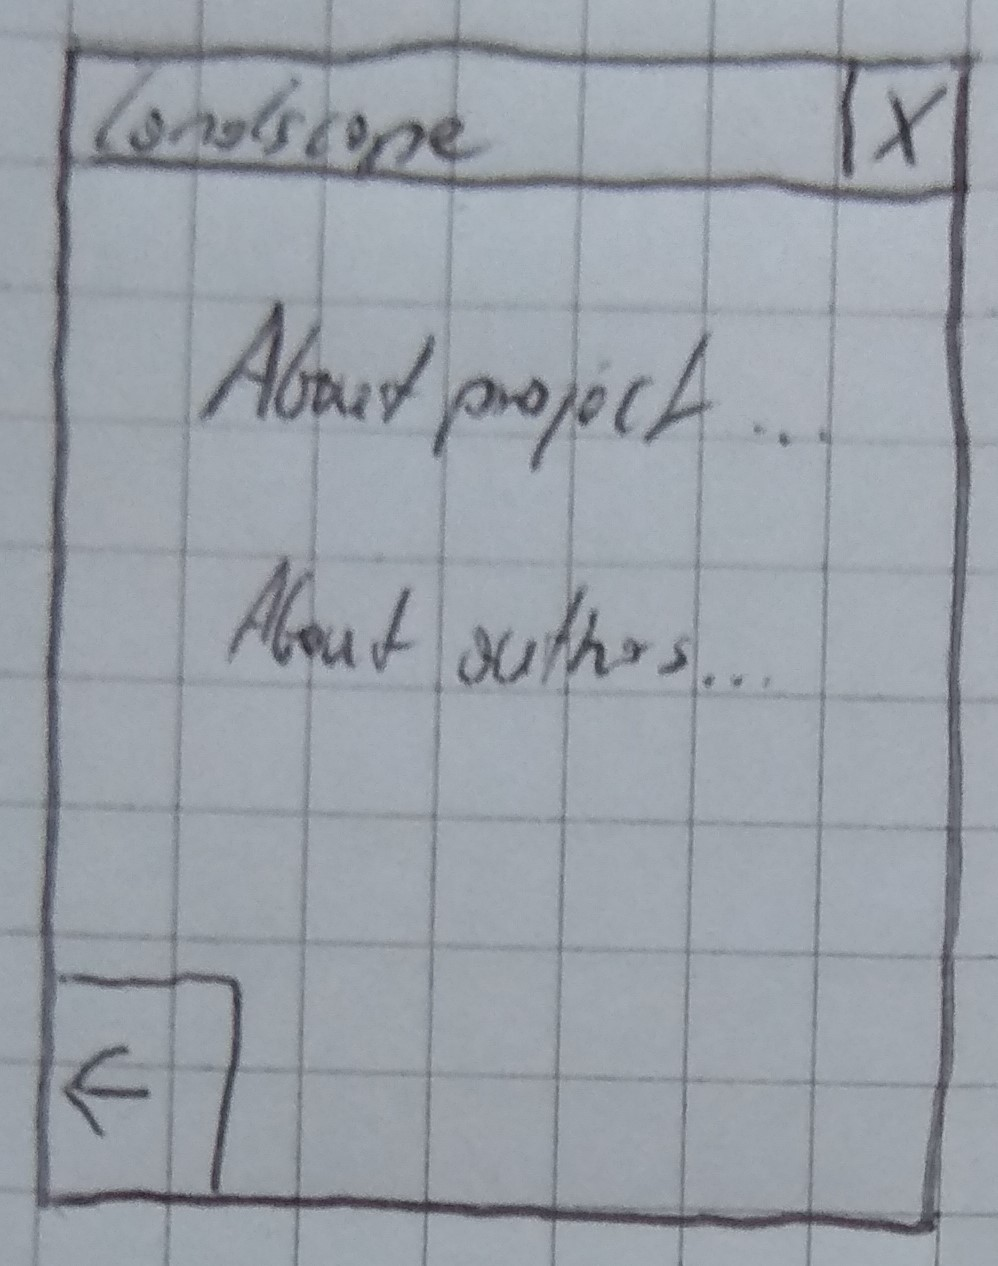
\includegraphics[width=0.5\textwidth]{Images/ui-about.jpg}
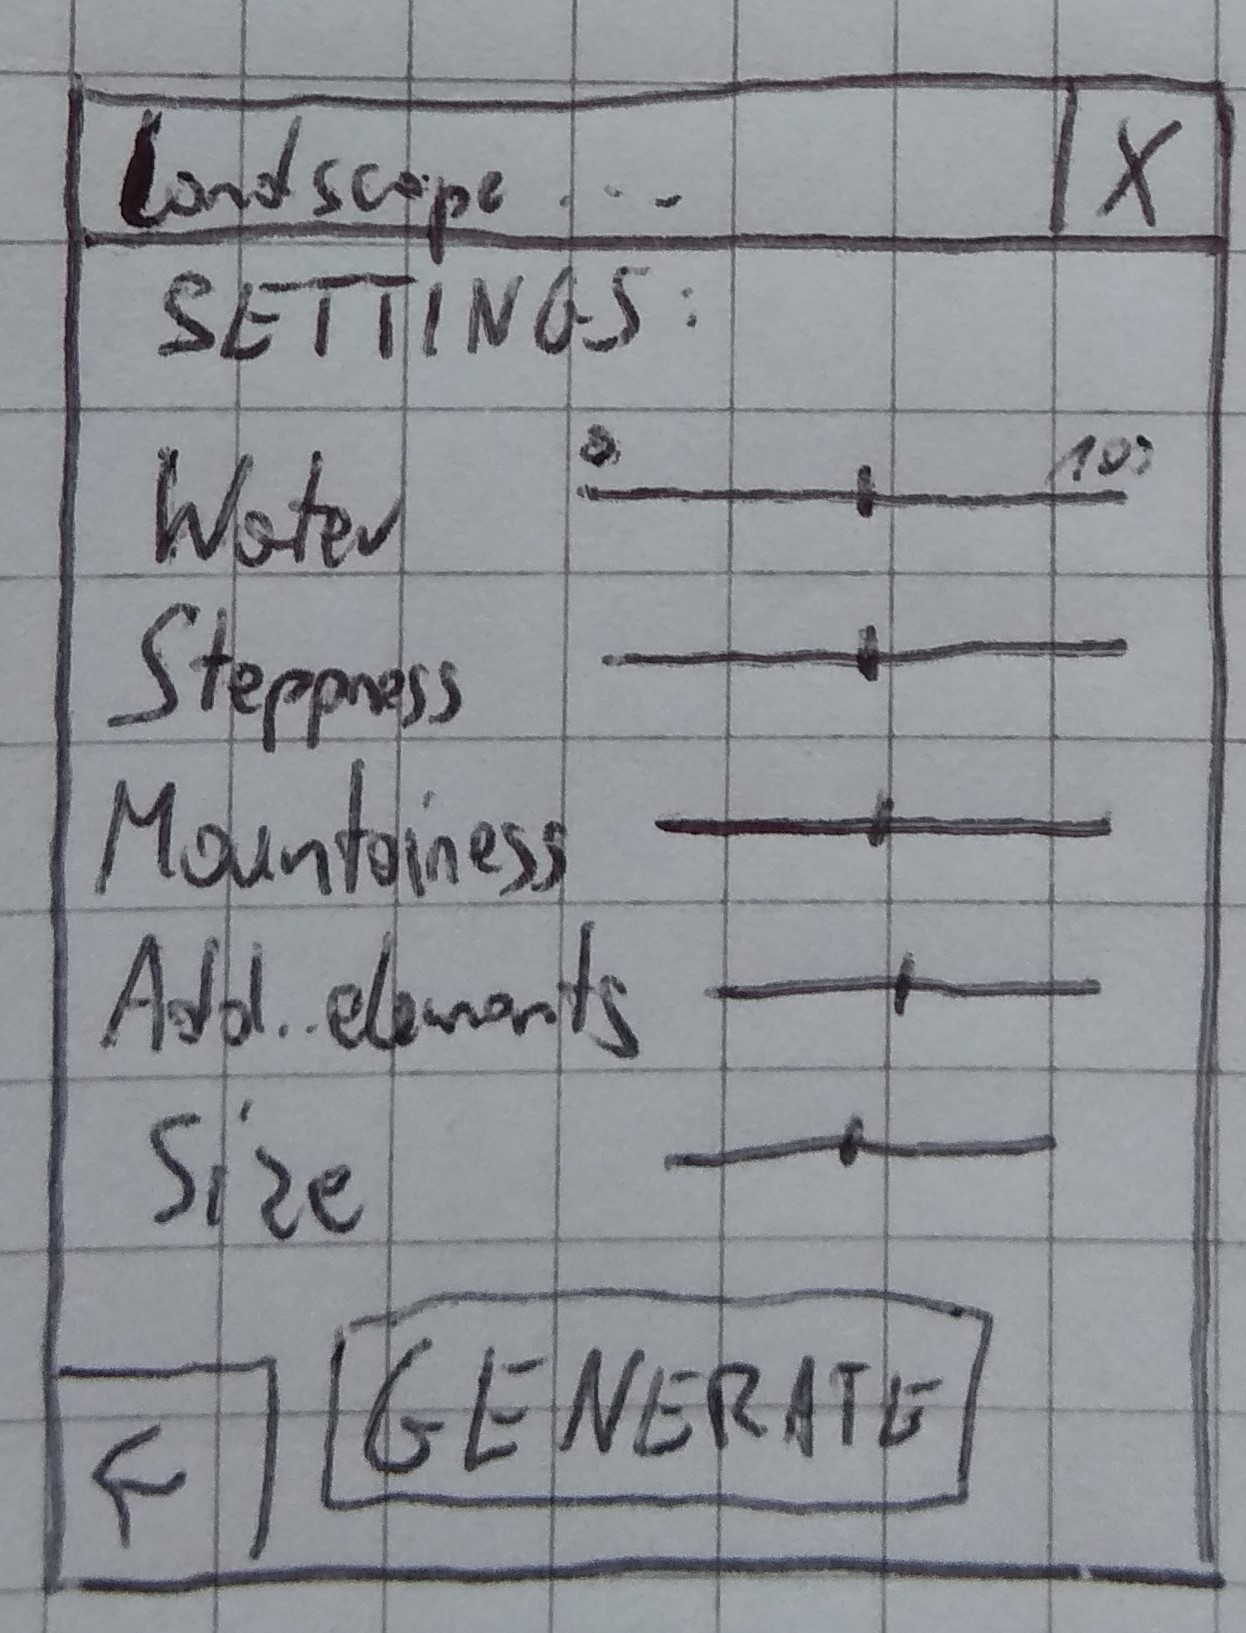
\includegraphics[width=0.5\textwidth]{Images/ui-settings.jpg}
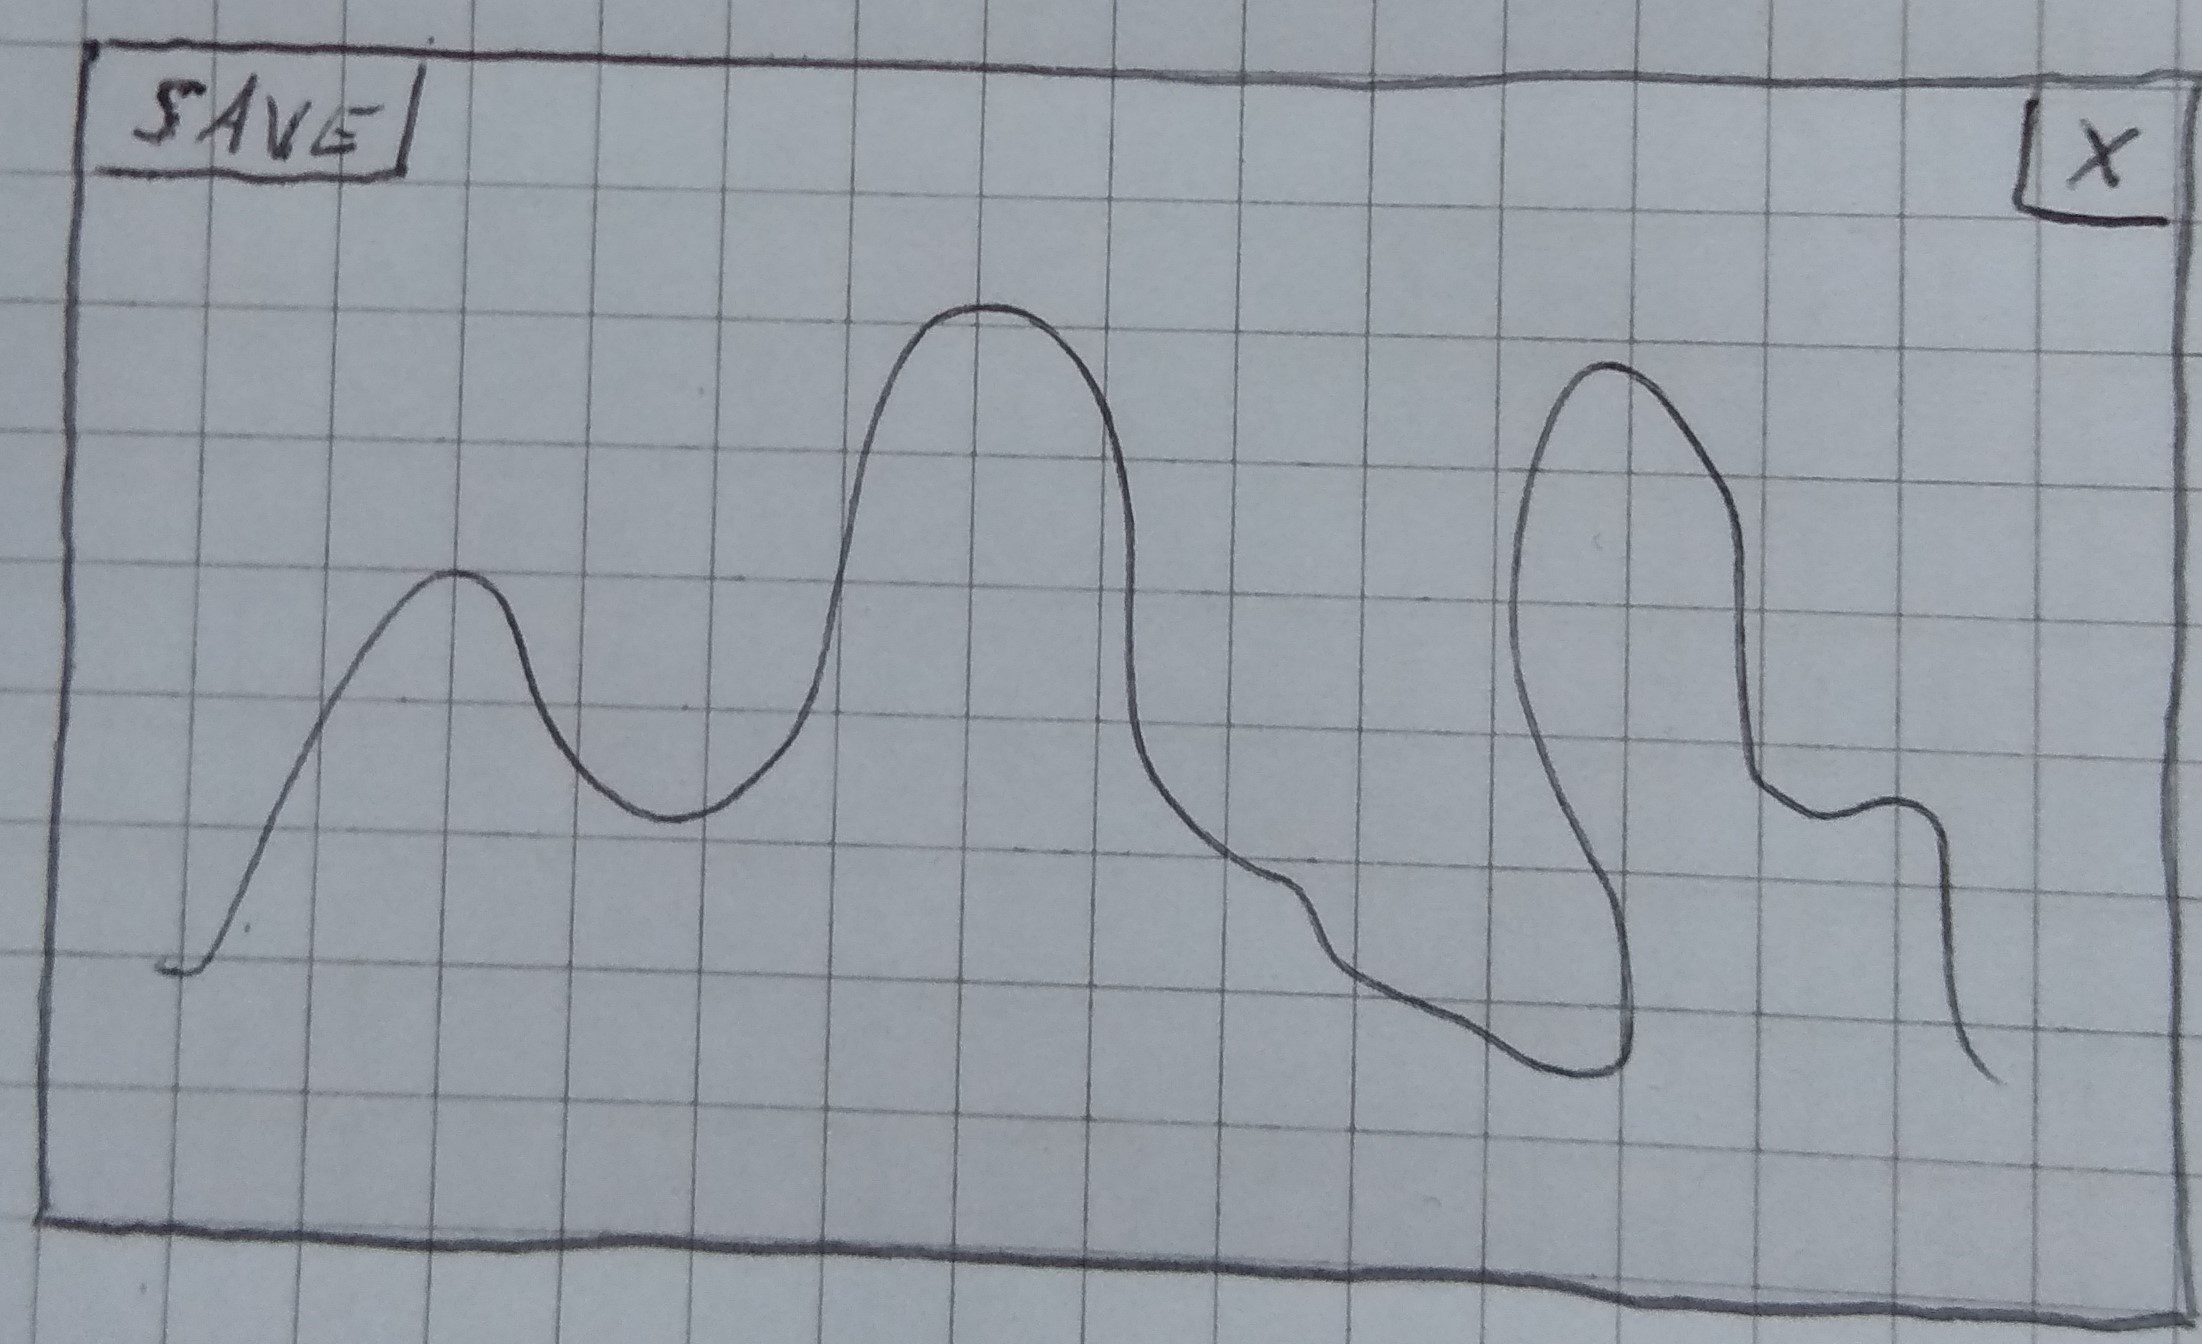
\includegraphics[width=0.5\textwidth]{Images/ui-landscape.jpg}
\section{Teoria}
\subsection{Losowość}
Celem projektu jest wygenerowanie losowego krajobrazu, więc sama losowość jest bardzo ważna. Każdy kolejny krajobraz powinien być inny, a prawdopodobieństwo wystąpienia dwóch podobnych obrazów bardzo niskie. Takie efekty możemy uzyskać dzięki algorytmowi jakim jest ,,Szum Perlina''
\subsection{Algorytmy}
\subsubsection{Szum Perlina}
Bazę dla naszego sposobu generowania danych potrzebnych do wyświetlenia zróżnicowanego terenu stanowi szum Perlina. Jest to jeden z typów szumu gradientowego utworzony przez Kena Perlina już w 1983 roku dla potrzeby tworzenia realistycznych grafik komputerowych. 
Algorytm składa się z trzech kroków
\begin{itemize}
\item Pierwszym krokiem jest zdefiniowanie wielowymiarowej siatki jednostkowych wektorów rozpatrywanego gradientu. W naszym przypadku są to wartości losowe z zakresu (0, 1) liczb rzeczywistych. Dla jednowymiarowego przypadku byłyby dostępne jedynie wartości -1 albo 1
\item Kolejno iteruje się po podawanych punktach. Punkt wpada do pewnej komórki wygenerowanej siatki. Następnie wyliczany jest iloczyn skalarny między punktem a wektorem każdego z rogów komórki (a więc ich odległość), po czym zapisane zostają w pamięci.
\item Przeprowadzona zostaje interpolacja dla każdej pary punktów z uwzględnieniem funkcji wygładzającej.
\end{itemize}
Wynikowo otrzymujemy wielowymiarową macierz (lub tensor) zawierający wartości zamknięte w pewnych granicach. Jest możliwe nakładanie na siebie wielu takich macierzy generowanych dla różnych częstotliwości siatki w celu uzyskania różnych ułożeń lub skupień wartości.
\section{Narzędzia}
\subsection{Kontrola wersji}
Do zarządzania kodem i wersjami projektu wykorzystujemy narzędzie Git. Korzystamy z platformy GitHub jako repozytorium dostępnego online. Dobór narzędzi służących do korzystania z repozytorium to sprawa indywidualna każdego członka zespołu, ponieważ nie ma ona wpływu na sam projekt.
\subsection{Zarzadzanie zespołem}
Trello - Kanban Board - to tutaj rozpisujemy zadania i przydzielamy je sobie, określamy również terminy i planujemy.
\subsection{Środowisko}
Visual Studio 2015 \\
Do wyświetlenia terenu wykorzystujemy zestaw funkcji API wspomagający generowanie grafiki – DirectX wraz z DirectX Software Development Kit używany z C\#.
\section{Aplikacja}
\subsection{Architektura}
\subsubsection{Silnik graficzny - InsightEngine}
Utworzony silnik graficzny jest wzorowany na istniejących już popularnych silnikach do gier takich jak Unity, Cry czy Unreal Engine. Opiera się on na trzech głównych składowych: \begin{itemize}
\item scena - obiekt nadrzędny, to w nim rozgrywa się akcja. Zawiera kolekcje encji.
\item encja - umieszczona w scenie. Jest to pojedynczy agent w scenie, np. kamera, teren czy postać. Zawiera kolekcje komponentów.
\item komponent - to składowa encji - odpowiada za część logiki encji (przykładowo, encja ``player`` może mieć komponenty takie jak ``moveComponent`` czy ``shootComponent``
\\
\end{itemize}
Silnik jest zbudowany zgodnie z wzrocem kompozytu - encja składa się z kompenentów, ale pojedynczy komponent może zawierać kolejne, zagnieżdżone komponenty. Pozwala to na rekurencyjne wykonywanie metod w obiektach o tym samym interfejsie. \\ \\
Z każdą kolejną wyświetlaną klatką scena wykonuje aktualizację wszystkich swoich encji, które aktualizują swoje komponenty. Pozwala to m.in. na ruch kamery. \\ \\
Specjalne komponenty typu ``Renderer`` klasy ``ShapeRenderer`` są odpowiedzialne za rysowanie na scenie obiektów 3D.


\subsubsection{Wygenerowany teren - TerrainGenerator}
Forma odpowiedzialna za wyświetlenie efektu działania silnika graficznego. Forma wywoływana jest z zestawem argumentów odpowiedzialnym za parametry generowanego terenu lub ścieżkę do pliku z zapisanym terenem.
\subsubsection{Generator terenu - PerlinNoise}
Klasa odpowiedzialna za generowanie kształtu terenu to PerlinNoise, implementuje interfejs INoiseGenerator. Ustawienia konfiguracyjne generatora znajdują się w folderze Config w plikach PerlinParameters oraz PerlinValueSetter.
Aby skorzystać z generatora należy utworzyć jego obiekt, który w konstruktorze wymaga rozmiaru generowanego obszaru i liczby wymiarów, w których liczymy. Następnie należy wywołać metodę CalculateNoiseValue, która jako argumenty przyjmuje współrzędne punktu oraz rozmiar mapy.
\subsubsection{Interfejs użytkownika - UI}
UI jest utworzone w projekcie WindowsForms. Zbudowane zgodnie z architekturą Model View Presenter. \begin{itemize}
\item VIEW - jedna forma odpowiedzialna za przełączanie między UserControl oraz utworzenie połączenia z prezenterami. Każdy obiekt UserControl jest umieszczony w osobnym folderze, gdzie posiada swój interfejs.
\item PRESENTER - każdy widok posiada tutaj swój odpowiedni folder, w którym znajduje się prezenter.
\item MODEL - model posiadający dane ENUM.
\end{itemize}
\subsubsection{Połączenie}
UI w momencie, gdy użytkownik chce wygenerować nowy lub wczytać z pliku teren, wywołuje formę TerrainGenerator, która wyświetli wynik pracy InsightEngine, który do generowania korzysta z PerlinNoise.
\subsection{Struktury danych}
Dane o wygenerowanym terenie będą przechowywane w pliku. Umożliwi nam to zapisanie i późniejsze odtworzenie terenu. Plik będzie przechowywał tablice odpowiadające za kształt terenu wraz z kolorami oraz drugą tablicę, która będzie przechowywać infromacje na temat położenia dodatkowych elementów wraz z typem danego elementu. Przykladowy plik:
\begin{lstlisting}[language=json,firstnumber=1]
[{x:y:z:c};{x:y:z:c}]
[{x:y:z:t};{x:y:z:t}]
\end{lstlisting}
Gdzie x,y,z to współrzędne, c to kolor, a t to tag odpowiadający za typ modelu.
\subsection{Schemat graficzny struktury systemu}
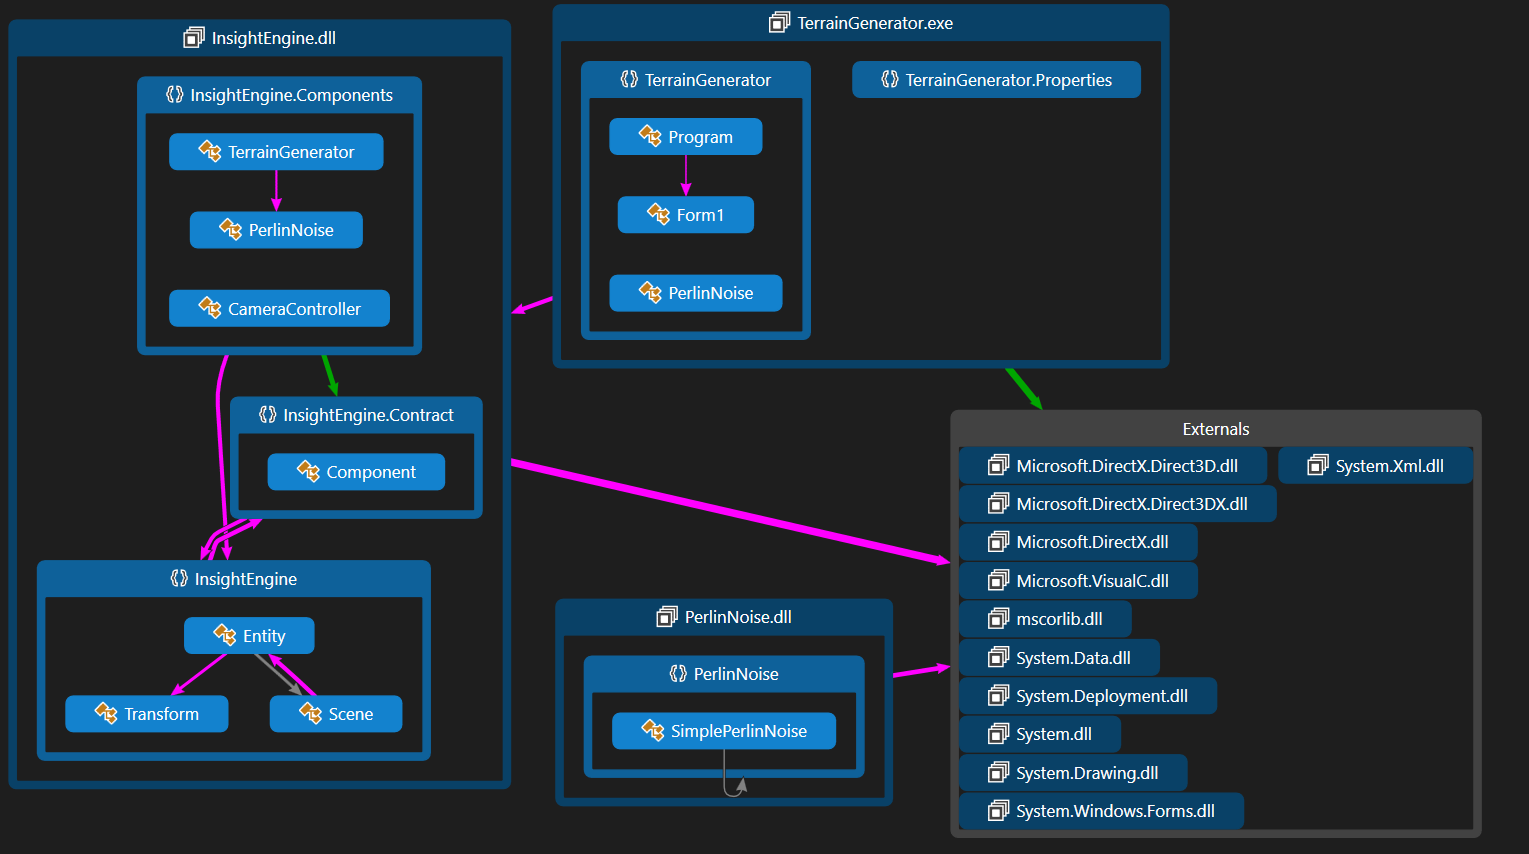
\includegraphics[width=1\textwidth]{images/klasy.png}
\section{API}
\subsection{PerlinNoise}
Konstruktor: PerlinNoise(int gradientSize, int numberOfDimensions) - gradientSize to rozmiar generowanego terenu, liczba wymiarów. Dla generatora 3D liczba wymiarów równa 3.\\
Pobranie wartości: CalculateNoiseValue(int x, int z, int Size) - x,z to współrzędne, Size to rozmiar generowanego terenu.
\subsection{InsightEngine}

\end{document}